\documentclass[10pt]{article}
\usepackage[margin=1in]{geometry}
\usepackage{graphicx}
\graphicspath{{./images/}}

\usepackage{amsmath, amssymb, amsthm, amsfonts, mathtools, bbm, breqn}
\usepackage{enumitem}       % for shortlabels
\usepackage{multicol}       % multiple columns
\usepackage{abraces}        % asymmetric braces
\usepackage{skull}
\usepackage{tikz}
\usetikzlibrary{arrows.meta, arrows, calc, matrix, positioning}

\usepackage{hyperref}
\usepackage[capitalize]{cleveref}


% Citing theorems by name. (source: https://tex.stackexchange.com/questions/109843/cleveref-and-named-theorems)
\makeatletter
\newcommand{\ncref}[1]{\cref{#1}\mynameref{#1}{\csname r@#1\endcsname}}

\def\mynameref#1#2{%
  \begingroup
  \edef\@mytxt{#2}%
  \edef\@mytst{\expandafter\@thirdoffive\@mytxt}%
  \ifx\@mytst\empty\else
  \space(\nameref{#1})\fi
  \endgroup
}
\makeatother

% for the pipe symbol
\usepackage[T1]{fontenc}

\usepackage{xcolor} % Enables a broader range of colors

% Define custom colors
\definecolor{RoyalBlue}{cmyk}{1, 0.50, 0, 0}

% Note commands
\definecolor{Red}{rgb}{1,0,0}
\definecolor{Blue}{rgb}{0,0,1}
\definecolor{Purple}{rgb}{.75,0,.25}
\newcommand{\rnote}[1]{\textcolor{Red}{[#1]}}       % Red note
\newcommand{\pnote}[1]{\textcolor{Purple}{[#1]}}    % Purple note
\newcommand{\bnote}[1]{\textcolor{Blue}{#1}}        % Blue text
\newcommand{\Max}[1]{\pnote{#1}}                    % Alias for purple note

% Emphasized text
\newcommand{\demph}[1]{\textcolor{RoyalBlue}{\textbf{\slshape #1}}} % Slanted RoyalBlue text


% Claim numbering (the counter restarts after each proof environment)
\newcounter{claimcount}
\setcounter{claimcount}{0}
\newenvironment{claim}{\refstepcounter{claimcount}\par\addvspace{\medskipamount}\noindent\textbf{Claim \arabic{claimcount}:}}{}
\usepackage{etoolbox}
\AtBeginEnvironment{proof}{\setcounter{claimcount}{0}}
\newenvironment{claimproof}{\par\addvspace{\medskipamount}\noindent\textit{Proof of Claim  \arabic{claimcount}.}}{\hfill\ensuremath{\qedsymbol} \tiny{Claim}

  \medskip}
% Add claim support to cleverref
\crefname{claimcount}{Claim}{Claims}

\usepackage[most]{tcolorbox} % for boxed text,
                             % use \begin{tcolorbox[width=0.7\linewidth,
                             % colback=white, colframe=black]}

\usepackage{empheq} % for boxed equations
\usepackage[most]{tcolorbox}
\newtcbox{\mymath}[1][]{%
  nobeforeafter, math upper, tcbox raise base,
  enhanced, colframe=blue!30!black,
  colback=blue!30, boxrule=1pt,
  #1}
\newtcbox{\boxmath}[1][]{%
  nobeforeafter, math upper, tcbox raise base,
  enhanced, colframe=blue!30!black,
  boxrule=1pt,
  #1}


\newenvironment{augmentedmatrix}[1] % environment for making augmented matrix
{\left[\begin{array}{#1}}
    {\end{array}\right]}



% Math Environments
\newtheorem{theorem}{Theorem}
\newtheorem{assumption}[theorem]{Assumption}
\newtheorem{lemma}[theorem]{Lemma}
\newtheorem{proposition}[theorem]{Proposition}
\newtheorem{corollary}[theorem]{Corollary}
\newtheorem{question}[theorem]{Question}
\theoremstyle{definition}
\newtheorem{definition}[theorem]{Definition}
\newtheorem{remark}[theorem]{Remark}
\newtheorem{example}[theorem]{Example}
\newtheorem{notation}[theorem]{Notation}
\newtheorem{problem}[theorem]{Problem}

% Redefine the Example environment to include "End of example [number]"
\makeatletter
\let\oldexample\example
\renewenvironment{example}
{\begin{oldexample}}
  {\par\smallskip\hfill   End of Example~\theexample. $\square$    \par\end{oldexample}}
\makeatother

% Custom Math Commands
\newcommand{\vt}{\vspace{5mm}}                       % Vertical space
\newcommand{\fl}[1]{\noindent\textbf{#1}}            % Bold first line
\newcommand{\Fl}[1]{\vspace{5mm}\noindent\textbf{#1}}% Bold first line with space above
\newcommand{\norm}[1]{\left\lVert #1 \right\rVert}   % Norm

% Common math symbols
\newcommand{\R}{\mathbb{R}}           % Real numbers
\newcommand{\N}{\mathbb{N}}           % Natural numbers
\newcommand{\C}{\mathbb{C}}           % Complex numbers
\newcommand{\Z}{\mathbb{Z}}           % Integers
\newcommand{\Q}{\mathbb{Q}}           % Rational numbers
\newcommand{\E}{\mathbb{E}}           % Expectation
\renewcommand{\P}{\mathbb{P}}         % Probability (renamed to avoid \P clash)
\newcommand{\indep}{\perp\!\!\!\perp} % Independence symbol

% Operators
\newcommand{\Var}{\mathrm{Var}}   % Variance
\newcommand{\tr}{\mathrm{tr}}     % Trace
\newcommand{\dist}{\mathrm{dist}} % Distance


\usepackage{biblatex}
\addbibresource{refs.bib}

\title{Lecture Notes for Math 307:\\Linear Algebra and Differential Equations}
\author{Instructor: Max Hill (Fall 2025)}
\date{Last updated: \today}
\begin{document}

\maketitle
\tableofcontents

\section*{About this document}

These lecture notes were prepared by Max Hill for a 16-week linear algebra course  (MATH
307) at University of Hawaii at Manoa in Fall 2025.

The textbook used is \textit{Linear Algebra and Differential Equations} (2002)
by G.~Peterson S.~Sochacki, in which we cover primarily Chapters 1,2,5, and 6


\newpage
\setcounter{section}{-1}
\section{Tentative Course Outline}

\begin{itemize}
  \item \textbf{Weeks 1-3: Matrices and determinants.} \textit{(Systems of linear
  equations, matrices, matrix operations, inverse matrices, special matrices
  and their properties, and determinants.)}
  \begin{itemize} 
    \item Section 1.1: Systems of Linear Equations
    \item Section 1.2: Matrices and Matrix Operations
    \item Section 1.3: Inverses of Matrices
    \item Section 1.4: Special Matrices and Additional Properties of Matrices
    \item Section 1.5: Determinants
    \item Section 1.6: Further Properties of Determinants
    \item Section 1.7: Proofs of Theorems on Determinants
  \end{itemize}

  \item \textbf{Weeks 4-6: Vector spaces.} \textit{(Vector spaces, subspaces, spanning
  sets, linear independence, bases, dimension, null space, row and column
  spaces, Wronskian.)}
  \begin{itemize}
    \item Section 2.1: Vector Spaces
    \item Section 2.2: Subspaces and Spanning Sets
    \item Section 2.3: Linear Independence and Bases
    \item Section 2.4: Dimension; Nullspace, Rowspace, and Column Space
    \item Section 2.5: Wronskians
  \end{itemize}
  \item \textbf{Weeks 7-11: Linear transformations, spectral theory.} \textit{(Linear
  transformation, eigenvalues and eigenvectors, algebra of linear
  transformations, matrices for linear transformations, eigenvalues and
  eigenvectors, similar matrices, diagonalization, Jordan normal form.)}
  \begin{itemize}
    \item Section 5.1: Linear Transformations
    \item Section 5.2: The Algebra of Linear Transformations
    \item Section 5.3: Matrices for Linear Transformations
    \item Section 5.4: Eigenvalues and Eigenvectors of Matrices
    \item Section 5.5: Similar Matrices, Diagonalization, and Jordan Canonical Form
    \item Section 5.6: Eigenvectors and Eigenvalues of Linear Transformations
  \end{itemize}
  \item \textbf{Midterm Exam}
  \item \textbf{Weeks 12-14: Systems of differential equations.} \textit{(Theory of
  systems of linear differential equations, homogeneous systems with constant
  coefficients, the diagonalizable case, nondiagonalizable case,
  nonhomogeneous linear systems, applications to $2\times 2$ and $3\times 3$
  systems of nonlinear differential equations.)}
  \begin{itemize}
    \item Section 6.1: The Theory of Systems of Linear Differential Equations
    \item Section 6.2: Homogenous Systems with Constant Coefficients: The
    Diagonalizable Case
    \item Section 6.3: Homogenous Systems with Constant Coefficients: The
    Nondiagonalizable Case
    \item Section 6.4: Nonhomogeneous Linear Systems
    \item Section 6.6: Applications Involving Systems of Linear Differential Equations
    \item Section 6.7: $2\times 2$ Systems of Nonlinear Differential Equations
  \end{itemize}
  \item \textbf{Weeks 14-16: Other stuff if time allows.} \textit{(Converting differential
  equations to first order systems (section 6.5), linearization of $2 \times 2$ nonlinear
  systems (???), stability and instability (section 6.7), predator-prey
  equations (section 6.7.1).)}
  \item \textbf{Final Exam}
\end{itemize}

\newpage
\section{2025-08-25 | Week 01 | Lecture 01}
\textit{This lecture is based on textbook section 1.1. Introduction to Systems
  of Linear Equations}

\begin{center}
  \begin{tcolorbox}[width=0.9\textwidth, colback=white, colframe=black]
    \textit{\textbf{The nexus question of this lecture:} What is a system of
      linear equations, and what does it mean to `solve' a system of linear
      equations?}
  \end{tcolorbox}
\end{center}

\subsection{A first example of a system of linear equations}
We begin with something concrete.


\begin{example}[A first example of a \textit{system of linear equations}]
  \label{ex:a-first-example-linear-system-equations}
  Consider the following word problem:

  \begin{quote}
    \textit{A boat travels between two ports on a river 48 miles apart. When traveling
      downstream (i.e., with the current), the trip takes 4 hours, but when
      traveling upstream (i.e., fighting the current), the trip takes 6 hours.}

    \textit{Assume that the boat and the current are both moving at a
      constant speed. What is the speed of the boat in still water, and what is
      the speed of the current?}
  \end{quote}
  This problem is hard to reason through without writing something down, but
  becomes much simpler when we formalize it mathematically with equations. The
  unknowns are (1) \textbf{the speed of the boat in still water} and (2)
  \textbf{the speed of the current}. So let
  \begin{align*}
    x &:= \text{(the speed of the boat in still water)}\\
    y &:= \text{(the speed of the current)}.
  \end{align*}
  The speed of the boat going downstream is $x+y$. Therefore, since
  $(\text{speed})\times (\text{time})= (\text{distance travelled})$, we have
  \begin{equation*}
    4(x+y)=48, \quad \text{or equivalently} \quad  x+y = 12.
  \end{equation*}
  Similarly, the sped of the boat going upstream is $x-y$, so
  \begin{equation*}
    6(x-y)=48, \quad \text{or equivalently} \quad  x-y = 8
  \end{equation*}
  Thus, we have the following \textit{system of linear equations:}
  \begin{equation}\label{eq:first-example-equations}
    \left\{ \begin{array}{l@{}l} x+y=12 \\x-y=8.  \end{array}\right.
  \end{equation}
  This system has \textbf{two equations} and \textbf{two variables} ($x$ and
  $y$).  You have encountered systems of equations like this many times.
  With the help of the technology of algebra, solving this problem (namely,
  solving System \eqref{eq:first-example-equations}) is much easier than solving the
  original word problem.

 
  \begin{itemize}
    \item In this case, the problem can be easily solved
    \textbf{algebraically} using a substitution (e.g., plug $x=8+y$ into the
    first equation and solve for $y$, then solve for $x$ after finding $y$).
    This gives the solution $(x,y) = (10,2)$. The speed of the boat in still
    water is 10mph. The speed of the river current is 2mph.
    \item We can conceive of another type of solution, which uses a
    \textbf{geometric}, rather than algebraic perspective: observe that each
    equation $x+y=12$ and $x-y=8$ represents a line on the $xy$-plane. Plot
    the lines. Their intersection is the point $(10,2)$, which is the
    solution.
    \item However, solving systems of equations like in
    \eqref{eq:first-example-equations} becomes more cumbersome when there are
    lots of variables and equations. Doing substitutions and algebraic
    manipulations will still work, but will be tedius and difficult if you
    have many equations and variables.

    Later, we will introduce a general algorithm which can solve any such
    system. This algorithm is called \demph{Gauss-Jordan elimination}, and it
    will be one of the core techniques that we will use to solve many types of
    problems in this class.
  \end{itemize}
\end{example}


\subsection{Key definitions: linear systems and their solutions}
In this section, we formalize the mathematical objects we are studying.

\begin{definition}[Linear equation]
  \label{def:linear-equation}
  A \demph{linear equation} in the variables $x_{1},\ldots,x_{n}$ is an
  equation that can be written in the form
  \begin{equation*}
    a_{1}x_{1}+a_{2}x_{2}+\ldots+a_{n}x_{n} = b,
  \end{equation*}
  where $a_{1},\ldots,a_{n}$ and $b$ are constants (e.g., fixed real numbers).
  The numbers $a_{1},\ldots,a_{n}$ are called \demph{coefficients}. 
\end{definition}

Note that the variables $x_{1},\ldots,x_{n}$ are not raised to any powers.
That's what makes the equation \textit{linear}. If we had squares or cubes of
some of the $x_{i}$'s, or products like $x_{1}x_{3}$, then the equation would
be quadratic or cubic, or something else, but not linear.

\begin{example}[Examples of linear equations]
  \label{ex:examples-linear-equations-first-examples}
  \begin{itemize}
    \item[]
    \item The equation
    \begin{equation*}
      2x-3y =1
    \end{equation*}
    is a linear equation in the variables $x$ and $y$. Its graph is a line on the
    $xy$-plane.
    \item The equation
    \begin{equation*}
      3x-y+2z = 9
    \end{equation*}
    is a linear equation in the variables $x,y$ and $z$. Its graph is a plane
    in 3-dimensional space (denoted $\R^{3}$).
    \item The equation
    \begin{equation*}
      -x_{1} +5 x_{2}+ \pi^{2} x_{3}+ \sqrt{2}x_{4} = e^{2}
    \end{equation*}
    is a linear equation in the variables $x_{1},x_{2},x_{3},$ and $x_{4}$.
    The coefficients are
    \begin{equation*}
      a_{1} = -1, \quad a_{2} = 5, \quad a_{3} = \pi, \quad \text{and} \quad a_{4}=\sqrt{2}.
    \end{equation*}
    The graph of this linear system is a 3-dimensional hyperplane in 4d-space
    (i.e., $\R^{4}$).

    \fl{Observation:} In these examples, we observe a simple relationship
    between the number of variables and the dimension of the graph:
    \begin{equation*}
      \text{(dimension of graph)} = (\text{\# of variables}) - 1.
    \end{equation*}
    Here, the term \demph{dimension} refers to the number of free variables.
    In the first equation (which is $2x-3y=1$), it's easy to see that if we
    know one of the variables, then the other one is automatically determined.
    So it makes sense that the graph of this equation is of dimension 1 (which
    it is, because it's a line). For the second equation, if we know any $2$
    of the variables, then the third variable is automatically determined, so
    it makes sense that the dimension of the graph is $2$ (which it is,
    because planes are 2-dimensional). Etc.
  \end{itemize}

\end{example}
\begin{definition}[Linear system, solution of a linear system]
  When considered together, a collection of $m$ linear equations
  \begin{equation}\label{eq:defn-system-of-linear-equations}
    \left\{ \begin{array}{l@{}l}
        \ a_{11}x_{1}+a_{12}x_{2}+\ldots+a_{1n}x_{n} = b_{1} \\
        \ a_{21}x_{1}+a_{21}x_{2}+\ldots+a_{2n}x_{n} = b_{2} \\
        \hfill\vdots\hfill \\
        a_{m1}x_{1}+a_{m2}x_{2}+\ldots+a_{mn}x_{n} = b_{m}
      \end{array}\right.
  \end{equation}
  is called a \demph{system of linear equations}, or \demph{linear system} for
  short. A \demph{solution} to a system of linear equations is a set of values
  for $x_{1},\ldots,x_{n}$ which satisfy all equations in
  system \eqref{eq:defn-system-of-linear-equations}.
\end{definition}

\begin{example}[A system of linear equations]
  \label{ex:system-linear-equations-first-example}
  An example of a system of linear equations is
  \begin{equation*}
    \left\{ \begin{array}{l@{}l}
        \hphantom{-2}x\; -\;  \hphantom{3}y \;+\;  \hphantom{4}z =\hphantom{-}0 \\
        \hphantom{-}2x\;-\; 3y\;+\; 4z= -2 \\
        -2x\;-\; \hphantom{3}y\;+\; \hphantom{4}z=\hphantom{-}7
      \end{array}\right.
  \end{equation*}
  When a linear system like this walks in the door, we always first ask two
  basic questions: (1) `how many equations does it have?' and (2) `how many
  variables does it have?'. In this case, we have $m=3$ equations and $n=3$
  variables.
\end{example}
\subsection{How to understand solutions of linear systems geometrically}
Here is a very useful geometric perspective. In
system \eqref{eq:defn-system-of-linear-equations}, we have a system of $m$ equations
expressed in $n$ variables $x_{1},\ldots,x_{n}$. Each of the $m$ equations is
the equation of some hyperplane\footnote{Note: Hyperplanes will be defined
  more formally later, but for now can be thought of as generalized lines or
  planes, since a 1-dimensional hyperplanes is a \textit{line} and a
  2-dimensional hyperplane is a \textit{plane}.} which lives in
$n$-dimensional space ($\R^{n}$). \textit{The solution to the linear system is the
  intersection of these hyperplanes.}

For example, in \cref{ex:system-linear-equations-first-example}, the
`hyperplanes' were lines, and their intersection was the point $(x,y)=(10,2)$.


We will spend a lot of time understanding what hyperplanes look like, and what
intersections of hyperplanes look like.



\newpage
\section{2025-08-27 | Week 01 | Lecture 02}

\begin{center}
  \begin{tcolorbox}[width=0.9\textwidth, colback=white, colframe=black]
    \textit{\textbf{The two main questions of this lecture:}
      \vspace{.5em}
      \begin{enumerate}
        \item How do we understand solutions of linear systems geometrically?
        \item How can we find a solution to a linear system algebraically,
        without resorting to substitution?
      \end{enumerate}}
  \end{tcolorbox}
\end{center}
\subsection{How to understand solutions of linear systems geometrically}
Here is a very useful geometric perspective. In
system \eqref{eq:defn-system-of-linear-equations}, we have a system of $m$ equations
expressed in $n$ variables $x_{1},\ldots,x_{n}$. Each of the $m$ equations is
the equation of some hyperplane\footnote{Note: Hyperplanes will be defined
  more formally later, but for now can be thought of as generalized lines or
  planes, since a 1-dimensional hyperplanes is a \textit{line} and a
  2-dimensional hyperplane is a \textit{plane}.} which lives in
$n$-dimensional space ($\R^{n}$). \textit{The solution to the linear system is the
intersection of these hyperplanes.}

The clearest example of this can be seen in the linear system:
\begin{equation}\label{eq:2x2-geometric-intuition-example}
  \left\{ \begin{array}{l@{}l}
      a_{11}x + a_{12}y = b_{1}\\
      a_{21}x + a_{22}y = b_{2}\\
    \end{array}\right.
\end{equation}
where $a_{12},a_{22}\neq 0$. (In this case, the ``hyperplanes'' are simply
lines.) Here, the solutions to the first equation are the points on the line
\begin{equation}\label{eq:line-1}
  y = -\frac{a_{11}}{a_{12}}x + b_{1}.
\end{equation}
Similarly, the solutions to the second equation are the points on the line
\begin{equation}\label{eq:line-2}
  y = - \frac{a_{21}}{a_{22}}x + b_{2}.
\end{equation}
There are three possible things that can happen when we intersect the two
lines in \cref{eq:line-1,eq:line-2}:
\begin{itemize}
  \item \textbf{Case 1.} The two line equations \cref{eq:line-1,eq:line-2}
  represent distinct lines and are not parallel. In this case, their
  intersection consists of a unique point, like this:
  \begin{center}
    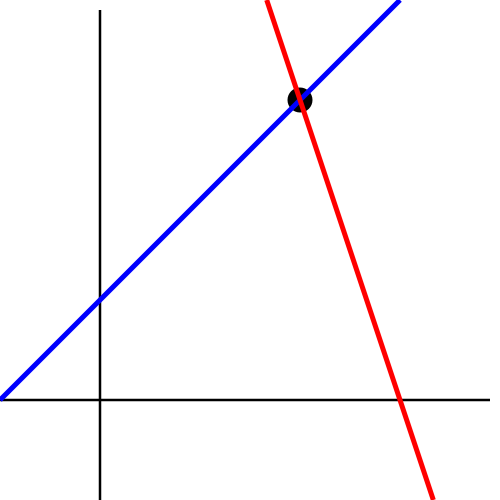
\includegraphics[scale=.12]{images/intersecting-lines} % wikipeida
  \end{center}
  In this case, the system \eqref{eq:2x2-geometric-intuition-example} has
  \textbf{exactly one solution}---namely, the intersection of the two lines,
  just like we saw in the boat example.
  
  \item \textbf{Case 2.} The two line equations \cref{eq:line-1,eq:line-2}
  represent two parallel but different lines. In this case, the two lines
  never intersect each other (i.e., there is no point that lies on both
  lines), so the system \eqref{eq:2x2-geometric-intuition-example} has
  \textbf{no solutions}.
  
  \item \textbf{Case 3.} The two equations of lines are the same, so they
  represent the same line. Therefore the intersection of the two lines is the
  entire line. Therefore, there are \textbf{infinitely many solutions} to the
  linear system \eqref{eq:2x2-geometric-intuition-example}. Namely, any point
  $(x,y)$ on the line is a solution to the linear system.
\end{itemize}
These three cases constitute the following trichotomy:


\begin{center}
  \begin{tcolorbox}[width=0.7\textwidth, colback=white, colframe=black]
    \textbf{Fact:} A system of linear equations either has (1) exactly one
    solution, (2) no solution, or (3) infinitely many solutions.
  \end{tcolorbox}
\end{center}

We haven't proven this fact, only illustrated it for systems of linear
equations like \eqref{eq:2x2-geometric-intuition-example} that have 2
equations and 2 variables. In fact, as we shall see, this fact always holds
for all linear systems of the form given in
\eqref{eq:defn-system-of-linear-equations}, no matter how many equations and
variables.

\subsection{Motivation for Gauss-Jordan Elimination}


\begin{center}
  \begin{tcolorbox}[width=0.9\textwidth, colback=white, colframe=black]
    \textit{\textbf{The nexus question for the rest of this lecture:} How can
      we solve a linear system without resorting to substitution?}
  \end{tcolorbox}
\end{center}

In the next lecture, I will present \demph{Gauss-Jordan elimination}, a
general algorithm which can be used to solve general systems of linear
equations, which does not use substitution. For now, I will answer the above
question by working out an example which motivates the main ideas, so that the
Gauss-Jordan algorithm doesn't feel like its coming out of nowhere when we
present it in the next lecture.
\begin{example}[Solving a linear system with elementary operations]
  \label{ex:solving-linear-system-with-elementary-operations}
  Suppose we wish to solve the following system:
  \begin{equation}
    \label{eq:elementary-operation-elimination-example}
    \left\{
      \begin{alignedat}{4}
        &x &{}\;-\; y &{}\;+\; &z{}&= &0 & \quad(E_{1}) \\ 
        2&x&{}\;-\; 3y&{}+\; 4&z{}&= -&2 & \quad(E_{2})\\
        -2&x&{}\;-\; y&{}\;+\; &z {}&= &7& \quad(E_{3})
      \end{alignedat}
    \right.
  \end{equation}
  This system has 3 equations, labeled $E_{1},E_{2},E_{3}$, and 3 variables
  $x,y$ and $z$. Suppose that we know ahead of time that this system has a
  unique solution (it does). Then, in principle, we could solve this using
  substitution, but that would suck. Instead, I will illustrate an approach in
  which we iteratively transform this linear system into successively simpler
  systems until we get to a point where the solution is obvious.

  To do this, we will play a game where there are three `moves' available to
  us. The three moves are:
  \begin{enumerate}
    \item Interchange two equations in the system.
    \item Multiply an equation by a nonzero number.
    \item Replace an equation by itself plus a multiple of another equation.
  \end{enumerate}
  These moves are called \demph{elementary operations}, and if we use them
  intelligently, they will allow us to transform the linear system into a
  simpler system.

  Two systems of equations are said to be \demph{equivalent} if they have the
  same solutions. Applying elementary operations always results in an
  equivalent system. Our goal will be to use some combination of elementary
  operations to produce a system of the form
  \begin{equation*}
    \left\{
      \begin{array}{l@{}l}
        x   &= *\\
        y &= *\\
        z &= *\\
      \end{array}\right.
  \end{equation*}
  where each $*$ is a constant which we will have computed. This will be our
  solution to the linear system \eqref{eq:elementary-operation-elimination-example},
  because the two systems will be equivalent.

  First, let's apply operation 3: specifically, by replacing $E_{2}$ with
  $E_{2} - 2E_{1}$:

\begin{equation*}
  \left\{
    \begin{alignedat}{4}
      &x &{}\;-\; y &{}\;+\; &z{}&= &0 \\
      & &{}\;-\; y&{}+\; 2&z{}&= -&2 \\
      -2&x&{}\;-\; y&{}\;+\; &z {}&= &7
    \end{alignedat}
  \right.
\end{equation*}
We have eliminated the $x$ from the second equation, yielding a simpler
system. Let's keep doing this. To eliminate $x$ from equation 3, let's apply
operation 3 again: This time, replace $E_{3}$ with $E_{3}+2 E_{1}$:
\begin{equation*}
  \left\{
    \begin{alignedat}{4}
      &x &{}\;-\; y &{}\;+\; &z{}&= &0 \\
      & &{}\;-\; y&{}+\; 2&z{}&= -&2 \\
      & &{}\; \; -3y&{}\;+\; 3&z {}&= &7
    \end{alignedat}
  \right.
\end{equation*}

Apply operation 3, replace $E_{1}$ with $E_{1}-E_{2}$. This will allow us to
eliminate $y$ from $E_{1}$:

\begin{equation*}
  \left\{
    \begin{alignedat}{4}
      &x &{}\;\;  &{}\;\; -&z{}&= &2 \\
      & &{}\;-\; y&{}+\; 2&z{}&= -&2 \\
      & &{}\; \; -3y&{}\;+\; 3&z {}&= &7
    \end{alignedat}
  \right.
\end{equation*}

Apply operation 3, replace $E_{3}$ with $E_{3}-3E_{2}$. This will allow us to
eliminate $y$ from $E_{3}$:
\begin{equation*}
  \left\{
    \begin{alignedat}{4}
      &x &{}\;\;  &{}\;\; -&z{}&= &2 \\
      & &{}\;-\; y&{}+\; 2&z{}&= -&2 \\
      & &{}\; \; &{}\;-\; 3&z {}&= &13
    \end{alignedat}
  \right.
\end{equation*}
Apply operation 2 twice: multiply both the first and second equations by $3$:
\begin{equation*}
  \left\{
    \begin{alignedat}{3}
      3x&   &{}\;\; -3&z{}= 6 \\
        & {}\;-\; 3y&{}\;+6&z{}= -6 \\
        & {}\; \; &{}\;\;- 3&z = 13
    \end{alignedat}
  \right.
\end{equation*}
Apply operation 3, twice. First, replace $E_{1}$ with $E_{1}-E_{3}$. Then
replace $E_{2}$ with $E_{2}+2E_{3}$. Doing both of these, we get:
\begin{equation*}
  \left\{
    \begin{alignedat}{3}
      3x \quad& &  & =&{} -7 \\
              & &3y \quad \quad& =&{} 20 \\
              & & -3z& =&{} 13
    \end{alignedat}
  \right.
\end{equation*}
Apply operation $2$ by dividing all three equations by $3$:
\begin{equation*}
  \left\{
    \begin{alignedat}{3}
      x \quad& &  & =&{} -7/3 \\
             & &y \quad \quad& =&{} 20/3 \\
             & & -z& =&{} 13/3
    \end{alignedat}
  \right.
\end{equation*}
This is the solution to the original equation. We have used elementary
operatons to reduce our original linear system
\cref{eq:elementary-operation-elimination-example} to the above system, which
equivalent to the original system.

While solving this system was still a lot of (tedious) work, it was still
probably simpler than doing substitution.
\end{example}

\begin{remark}[Forget the variables]
  In the procedure presented in , we didn't really need to track the variables, only
  the \textit{coefficients} and the \textit{quantities on the right hand sides} of the
  equations. Instead of working with the equations directly, it will be
  simpler to work with the following matrix, called the \demph{augmented
    matrix} corresponding go \cref{eq:elementary-operation-elimination-example}:
  \begin{equation*}
    \begin{augmentedmatrix}{ccc|c}
      1& -1& 1& 0 \\
      2& -3& 4& -2 \\
      -2& -1& 1& 7
    \end{augmentedmatrix}.
  \end{equation*}
\end{remark}
Comparing this with system \eqref{eq:elementary-operation-elimination-example}, it becomes
clear that the augmented matrix was obtained essentially by just erasing the
variables $x,y,$ and $z$ in \eqref{eq:elementary-operation-elimination-example}, and
then placing what remains into an array. We also drew a vertical line to the
separate the left- and right-hand sides of the equations. Inside the augmented
matrix, the $3\times 3$ submatrix  of coefficients
\begin{equation*}
  \begin{bmatrix}
    1& -1& 1\\
    2& -3& 4\\
    -2& -1& 1
  \end{bmatrix}
\end{equation*}
is called the \demph{coefficient matrix} of the system. 

More precise definitions are as follows:

\begin{definition}[Augmented Matrix]
  Given a linear system of the form \eqref{eq:defn-system-of-linear-equations},
  the \demph{augmented matrix} is
  \begin{equation*}
    \begin{augmentedmatrix}{cccc|c}
      a_{11}&a_{12}&\ldots& a_{1n}& b_{1}\\
      a_{21}&a_{22}&\ldots& a_{2n}& b_{2}\\
      \vdots &\vdots & &\vdots &\vdots \\
      a_{m1}&a_{m2}&\ldots& a_{mn}& b_{m}
    \end{augmentedmatrix}
  \end{equation*}
  and the \demph{coefficient matrix} is the matrix
  \begin{equation*}
    \begin{bmatrix}
      a_{11}&a_{12}&\ldots& a_{1n}\\
      a_{21}&a_{22}&\ldots& a_{2n}\\
      \vdots&\vdots & &\vdots \\
      a_{m1}&a_{m2}&\ldots& a_{mn}
    \end{bmatrix}.
  \end{equation*}
\end{definition}
\newpage
\section{2025-08-29 | Week 01 | Lecture 03}
\begin{center}
  \begin{tcolorbox}[width=0.9\textwidth, colback=white, colframe=black]
    \textit{\textbf{The nexus question of this lecture:} What is Gauss-Jordan Elimination?}
  \end{tcolorbox}
\end{center}

\Fl{Steps:} We initialize the algorithm by setting up an \demph{augmented
  matrix} corresponding to the system. For the system in
\eqref{eq:Gauss-Jordan-elimination-example}, the augmented matrix is
\begin{equation*}
  \begin{augmentedmatrix}{ccc|c}
    1& -1& 1& 0 \\
    2& -3& 4& -2 \\
    -2& -1& 1& 7
  \end{augmentedmatrix}.
\end{equation*}

\begin{itemize}
  \item The matrix to the left of the vertical row is called the
  \demph{coefficient matrix.}
  \item A line of numbers going from left to right is called a \demph{row} of the
  matrix. A line of numbers going down the matrix is a \demph{column.}
\end{itemize}



Gauss-Jordan elimination is like a game where the player has three possible
moves, called \demph{row operations}:
\begin{enumerate}
  \item Interchange two rows.
  \item Multiply a row by a nonzero number.
  \item Replace a row by itself plus a multiple of another row.
\end{enumerate}
The player does row operations with the \textbf{goal} of making as many
numbers in the coefficient matrix zero as possible.


\begin{equation*}
  \begin{augmentedmatrix}{ccc|c}
    1& -1& 1& 0 \\
    2& -3& 4& -2 \\
    -2& -1& 1& 7
  \end{augmentedmatrix}
  \overset{R_{2}-2R_{1}}{\longrightarrow}
  \begin{augmentedmatrix}{ccc|c}
    1& -1& 1& 0 \\
    \mathbf{0}& \mathbf{-1}& \mathbf{2}& \mathbf{-2} \\
    -2& -1& 1& 7
  \end{augmentedmatrix}
  \overset{R_{3}+2R_{1}}{\longrightarrow}
  \begin{augmentedmatrix}{ccc|c}
    1& -1& 1& 0 \\
    0& -1& 2& -2 \\
    \mathbf{0}& \mathbf{-3}& \mathbf{3}& \mathbf{7}
  \end{augmentedmatrix}
\end{equation*}
\begin{equation*}
  \overset{R_{1}-R_{2}}{\longrightarrow}
  \begin{augmentedmatrix}{ccc|c}
    \mathbf{1}& \mathbf{0}& \mathbf{-1}& \mathbf{2} \\
    0& -1& 2& -2 \\
    0& -3& 3& 7
  \end{augmentedmatrix}
  \overset{R_{3}-3R_{2}}{\longrightarrow}
  \begin{augmentedmatrix}{ccc|c}
    1& 0& -1& 2 \\
    0& -1& 2& -2 \\
    \mathbf{0}& \mathbf{0}& \mathbf{-3}& \mathbf{13}
  \end{augmentedmatrix}
  \overset{(-1)\cdot R_{2}}{\longrightarrow}
  \begin{augmentedmatrix}{ccc|c}
    1& 0& -1& 2 \\
    \mathbf{0}& \mathbf{1}& \mathbf{-2}& \mathbf{2} \\
    0& 0& -3& 13
  \end{augmentedmatrix}
\end{equation*}
\begin{equation*}
  \overset{(-\frac{1}{3})\cdot R_{3}}{\longrightarrow}
  \begin{augmentedmatrix}{ccc|c}
    1& 0& -1& 2 \\
    0& 1& -2& 2 \\
    \mathbf{0}& \mathbf{0}& \mathbf{1}& \mathbf{-13/3}
  \end{augmentedmatrix}
  \overset{R_{2}+2R_{3}}{\longrightarrow}
  \begin{augmentedmatrix}{ccc|c}
    1& 0& -1& 2 \\
    \mathbf{0}& \mathbf{1}& \mathbf{0}& \mathbf{-20/3} \\
    0& 0& 1& -13/3
  \end{augmentedmatrix}
  \overset{R_{1}+R_{3}}{\longrightarrow}
  \begin{augmentedmatrix}{ccc|c}
    \mathbf{1}& \mathbf{0}& \mathbf{0}& \mathbf{-7/3} \\
    0& 1& 0& -20/3 \\
    0& 0& 1& -13/3
  \end{augmentedmatrix}
\end{equation*}
We now convert the augmented matrix back to a system of linear equations:
\begin{equation*}
  \left\{
    \begin{alignedat}{4}
      &1x &{}\;-\; 0y &{}\;+\; &0z{}&= -&7/3 \\
      &0x&{}\;-\; 1y&{}\;+\; &0z{}&= -&20/3 \\
      &0x&{}\;-\; 0y&{}\;+\; &1z {}&= -&13/3
    \end{alignedat}
  \right.
\end{equation*}
or more simply,
\begin{align*}
  x &= -7/3\\
  y &= -20/3\\
  z &= -13/3
\end{align*}
We can check that this is a solution to the original system of equations \eqref{eq:Gauss-Jordan-elimination-example}.
\end{document}